\let\negmedspace\undefined
\let\negthickspace\undefined
\documentclass[journal]{IEEEtran}
\usepackage[a5paper, margin=10mm, onecolumn]{geometry}
%\usepackage{lmodern} % Ensure lmodern is loaded for pdflatex
\usepackage{tfrupee} % Include tfrupee package

\setlength{\headheight}{1cm} % Set the height of the header box
\setlength{\headsep}{0mm}     % Set the distance between the header box and the top of the text

\usepackage{gvv-book}
\usepackage{gvv}
\usepackage{cite}
\usepackage{amsmath,amssymb,amsfonts,amsthm}
\usepackage{algorithmic}
\usepackage{graphicx}
\usepackage{textcomp}
\usepackage{xcolor}
\usepackage{txfonts}
\usepackage{listings}
\usepackage{enumitem}
\usepackage{mathtools}
\usepackage{gensymb}
\usepackage{comment}
\usepackage[breaklinks=true]{hyperref}
\usepackage{tkz-euclide} 
\usepackage{listings}
% \usepackage{gvv}                                        
\def\inputGnumericTable{}                                 
\usepackage[latin1]{inputenc}                                
\usepackage{color}                                            
\usepackage{array}                                            
\usepackage{longtable}                                       
\usepackage{calc}                                             
\usepackage{multirow}                                         
\usepackage{hhline}                                           
\usepackage{ifthen}                                           
\usepackage{lscape}
\begin{document}

\bibliographystyle{IEEEtran}
\vspace{3cm}

\title{9-9.2-20}
\author{EE24BTECH11066 - YERRA AKHILESH
}
% \maketitle
% \newpage
% \bigskip
{\let\newpage\relax\maketitle}

\renewcommand{\thefigure}{\theenumi}
\renewcommand{\thetable}{\theenumi}
\setlength{\intextsep}{10pt} % Space between text and floats


\numberwithin{equation}{enumi}
\numberwithin{figure}{enumi}
\renewcommand{\thetable}{\theenumi}
\textbf{Question}:\\
Find the area of the region bounded by the curves $y = x^2+2$ $y = x$, $x = 0$ and $x = 3$.
\\
\textbf{solution: }
\begin{table}[h!]
    \centering
    \begin{tabular}[12pt]{ |c| c|}
    \hline
    \textbf{M} & $\nu$ \textbf{(Prandtl-Meyer function)}\\ 
    \hline
    1.8 & 20.73 \\
    \hline
    1.9 & 23.59 \\
    \hline
    2.0 & 26.38 \\
    \hline
    2.1 & 29.10 \\
    \hline
    2.2 & 31.73 \\
    \hline
    2.3 & 34.28 \\
    \hline
    2.4 & 36.75 \\
    \hline
    \end{tabular}
\end{table}
The parameters of the conic are\\
\begin{table}[h!]
    \centering
    \begin{tabular}[12pt]{ |c| c|}
    \hline
    \textbf{Conic}& \textbf{Parameters}\\ 
    \hline
     $V$& $\myvec{0 & 0 \\ 0 & 1}$\\
    \hline 
     $u$& $\frac{-1}{2}\myvec{1\\0}$\\
    \hline
     $f$& $0$\\
     \hline
    \end{tabular}
    \label{Table2}
\end{table}

The equation of a parabola in Matrix form is
\begin{align}
\vec{x}^\top\vec{V}\vec{x} + 2\vec{u}^\top\vec{x} + f = 0
\end{align}
The equation of a line in vector form is
\begin{align}
\vec{x}&=\vec{h}+\kappa\vec{m}
\end{align}
For the given parabola $y=x^2+2$, The values of $\vec{V}$,$\vec{u}$,$f$ are
\begin{align}
\vec{V}&=\myvec{1 & 0\\0 & 0}\\
\vec{u}&=\myvec{0\\\frac{-1}{2}}\\
f&=-2
\end{align}
For the given line $x=0$, The values of $\vec{h_1}$, $\vec{m_1}$ are
\begin{align}
\vec{h_1}&=\myvec{0\\0}\\
\vec{m_1}&=\myvec{0\\1}
\end{align}
Substituing $x=0$ line equation in parabola equation gives the values of $\kappa$
\begin{align}
\brak{\vec{h}+\kappa\vec{m}}^\top\vec{V}\brak{\vec{h}+\kappa\vec{m}} + 2\vec{u}^\top\brak{\vec{h}+\kappa\vec{m}} + f &= 0\\
\brak{\myvec{0\\0}+\kappa\myvec{0\\1}}^\top\myvec{1 & 0\\0 & 0}\brak{\myvec{0\\0}+\kappa\myvec{0\\1}} + 2\myvec{0\\\frac{-1}{2}}^\top\brak{\myvec{0\\0}+\kappa\myvec{0\\1}} + -2 &= 0\\
\myvec{\kappa&\kappa}\myvec{1&0\\0&0}\myvec{\kappa\\\kappa}+2\myvec{0&\frac{-1}{2}}\myvec{\kappa\\\kappa} &= 2\\
\myvec{\kappa&\kappa}\myvec{\kappa\\0}-\brak{\kappa} &= 2\\
\kappa^2-\kappa &= 2\\
\kappa_1&=2\\
\kappa_2&=-1
\end{align}
The intersection points are
\begin{align}
\vec{x_1} &= \vec{h}+\kappa_1\vec{m}\\
\vec{x_1} &= \myvec{0\\2}
\end{align}
as $k_2$ is negative so we neglect that point of intersection.\\
similarly for $x=3$ line intersection points are
\begin{align}
    \vec{x_2} &= \myvec{3\\11}
\end{align}
The Area under the curve $y=x^2+2$ is given by
\begin{align}
A_1 &= \int_{0}^{3}\brak{x^2+2}dx\\
A_1 &= \brak{\frac{x^3}{3} + 2x} \Big|_0^3\\
A_1 &= \brak{\frac{3^3}{3} + 2\cdot 3} - \brak{0}\\
A_1 &= \brak{9 + 6}\\
A_1 &= 15
\end{align}
The Area under the line $y=x$ is given by
\begin{align}
A_2 &= \int_{0}^{3}\brak{x}dx\\
A_2 &= \brak{\frac{x^2}{2}} \Big|_0^3\\
A_2 &= \frac{3^2}{2} - 0\\
A_2 &= \frac{9}{2}\\
A_2 &= 4.5
\end{align}
The area of region bounded by the line $x=y$ and the parabola $y=x^2+2$ is given by
\begin{align}
A &= A_1-A_2\\
A &= 15 - 4.5\\
A &= 10.5
\end{align}
The area of region bounded by the line $x=y$ and the parabola $y=x^2+2$ is $10.5$.
\begin{figure}[htp]
    \centering
    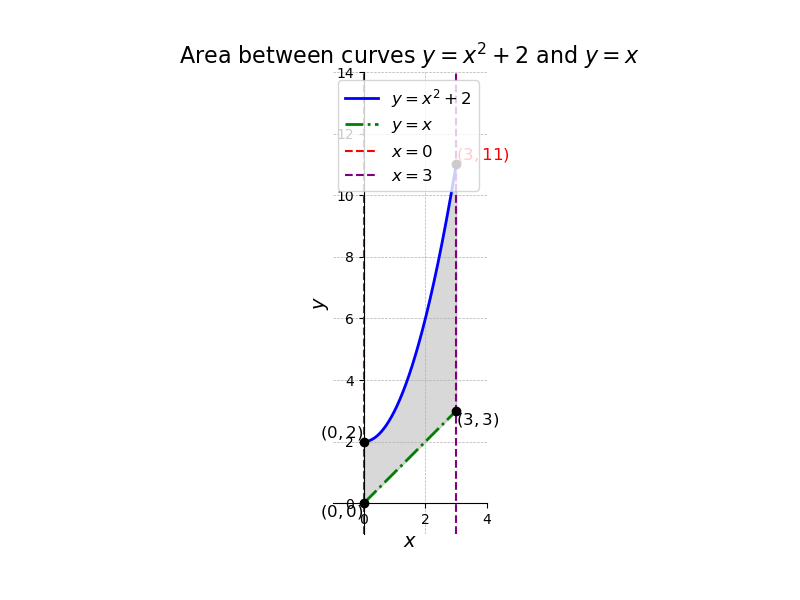
\includegraphics[width=10cm]{figs/Figure_1.png}
\end{figure}
\end{document}










